\documentclass[a4paper]{article}
\usepackage{listings}
\usepackage{xcolor}
\usepackage {fontspec}
\usepackage{fancyhdr}	
\pagestyle{fancy}
\setromanfont{Lantinghei SC Extralight}
\setmonofont{Courier New}
\XeTeXlinebreaklocale ``zh''
\XeTeXlinebreakskip = 0pt plus 1pt
\textheight = 650pt
\lstset{
	%行号
   numbers=left,
  %背景框
   framexleftmargin=10mm,
   frame=none,
   %背景色
   %backgroundcolor=\color[rgb]{1,1,0.76},
   backgroundcolor=\color[RGB]{245,245,244},
   %样式
   keywordstyle=\bf\color{blue},
   identifierstyle=\bf,
   numberstyle=\tiny,
   numberstyle=\color[RGB]{0,192,192},
   commentstyle=\it\color[RGB]{0,96,96},
   stringstyle=\rmfamily\slshape\color[RGB]{128,0,0},
   %显示空格
   showstringspaces=false
 }

\begin{document}
\title{实验报告 实验六}
\author{姓名:王钦\quad 学号:13349112\quad 班级:计科二班}
\date{}

\maketitle
\section*{ 实验目的}
\hangindent=4em \hangafter=-10{
  1. 学习进程模型知识,掌握进程模型的实现方法。\\
  2. 利用时钟中断,设计时钟中断处理进行进程交替执行\\
  3. 扩展MyOS,实现多进程模型的原型操作系统\\
}
\section*{ 实验内容}
\hangindent=4em \hangafter=-10{
在实验五的基础上,进化你的原型操作系统,原型保留原有特征的基础上,设计满足下列要求的新原型操作系统:\\
(1)内核实现简单进程模型,进程具有就绪、运行两种基本状态。建议在c程序中定义进程表,进程数量最多4个。\\
(2)内核可以一次性加载最多4个用户程序。用户进程采用时间片轮转调度进程。由你设计有个性的用户程序,它们的输出各占1/4屏幕区域,信息输出有动感,以便观察程序是否在执行。\\
(3)在原型中保证原有的系统调用服务可用。再编写4个用户程序,展示系统调用服务还能工作。\\
}

\section*{ 实验平台}
\hangindent=4em \hangafter=-10{
  dd+gcc+ld+nasm+Linux+vim\\
}

\section*{ 算法流程图}
\hangindent=4em \hangafter=-10{
  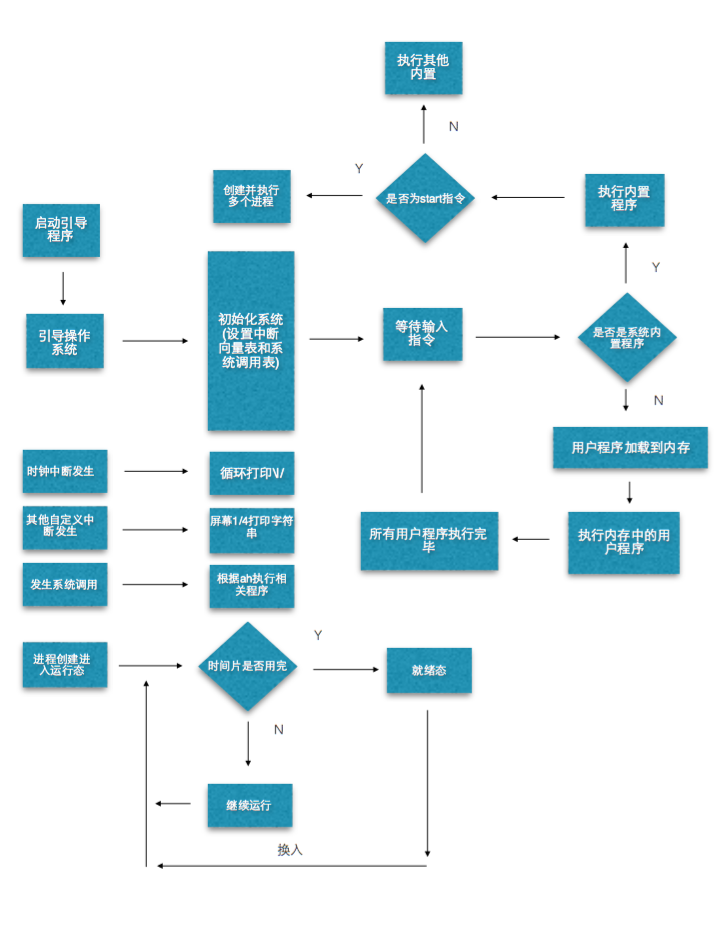
\includegraphics[scale=0.45]{Illustrations/flow.png}
}

\section*{ 功能一览}
\hangindent=4em \hangafter=-50{
	{\large 1. 系统内置功能:}\\
		\indent \verb| terminal|,装载内核shell,为用户提供一个与操作系统交互的工具,开机后自动进入,以下所有功能都在terminal中交互\\
		\indent	\verb| date|, 显示当前日期\\
		\indent \verb| time|, 显示当前时间\\
		\indent \verb| asc|, 显示一个字符的asc码\\
		\indent \verb| clear|, 清除当前屏幕所有字符,刷新屏幕\\
		\indent \verb| help|, 显示系统帮助信息\\
		\indent \verb| man |, 显示内置函数的帮助信息,比如\verb| man date |,显示date的相关帮助\\
		\indent \verb| python |, python 扩展,类似python命令行工具,可以使用这个工具输入计算表达式返回计算结果,目前只支持加法减法\\
		\indent \verb| start|, 开始创建并执行四个进程并且每秒18.2次的调度,分别在屏幕\verb|1/4|处打印一些个性化信息( 不同配置的虚拟机动画速度不一样,建议使用vmware测试)\\\\
	{\large 2. 用户程序:}\\
		\indent \verb| run |,软盘中含有两个用户程序,输入\verb|run 12|,可分别执行两个用户程序,当然也可以通过改变执行序列来改变执行的顺序\\\\
	{\large 3. 自定义中断:}\\
		\indent 时钟中断:通过PTR每秒发出18.2次的信号来从8592芯片的RT0引脚发出终端号\verb|int 08h|来触发的用户时钟软中断\verb| int 1ch|,实现在\verb|terminal|的右下角
	  一个横杠在转动.\\
		\indent 另外有自定义中断\verb|int 33h,int 34h,int 35h,int 36h|分别在屏幕四分之一的位置打印个性化信息\\\\
	{\large 4. 进程调度:}\\
		\indent 软盘中共存放了用于展示进程调度的五个应用程序,其中一个应用程序为监听用户键盘事件然后退出多进程调度状态回到\verb| terminal|每个应用程序分别代表一个进程。开启装载进程并进行进程调度由\verb|1|中系统内置功能的\verb| start|指令激活。\\
}

\section*{ 实验步骤及效果图}
\hangindent=4em \hangafter=-50{
1. 编辑修改ASM 文件,和C文件	\\\\
2. 使用make命令配合\verb|makefile|文件进行编译	\\\\
3. 运行\verb|bochs or vmware|虚拟机进行测试,进入后所看到的欢迎界面,同时进入terminal界面等待输入指令
{\center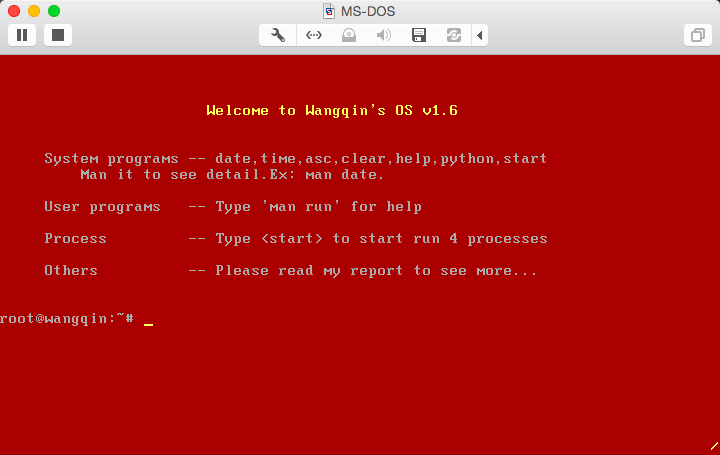
\includegraphics[scale=0.45]{Illustrations/start.png}}\\\\
4. 我们可以执行\verb|man python |\\查看\verb|python|的作用,主要功能是输入一个数学表达式然后返回表达式的结果,类似\verb|python|命令行的作用。其他类似的系统内置功能也可以使用\verb|man|命令来查看帮助信息。
但目前\verb|python|只支持加法和减法且只能有两个操作数(其实主要为了展示\verb|ah=3,4|将字符串转为数值和将数值转为字符串的系统调用效果),我这里仿照\verb|linux|系统的系统调用,设置
\verb|int 80h |为所有系统调用的入口。可以看到图中分别输入加法减法,返回计算结果。如果输入的不符合格式就会返回错误提示。最后输入\verb|exit|退出\verb|python|命令行工具。
{\center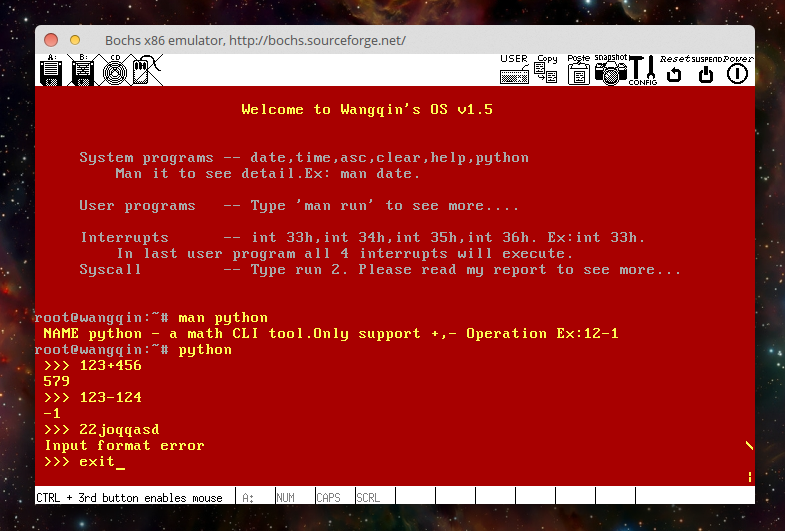
\includegraphics[scale=0.45]{Illustrations/python.png}}\\\\
5. 接下来测试ah等于\verb|0,1,2,5|的系统调用(显示\verb|OUCH|,字母大小写变化等),输入\verb| run 2 |,运行第二个用户程序,
{\center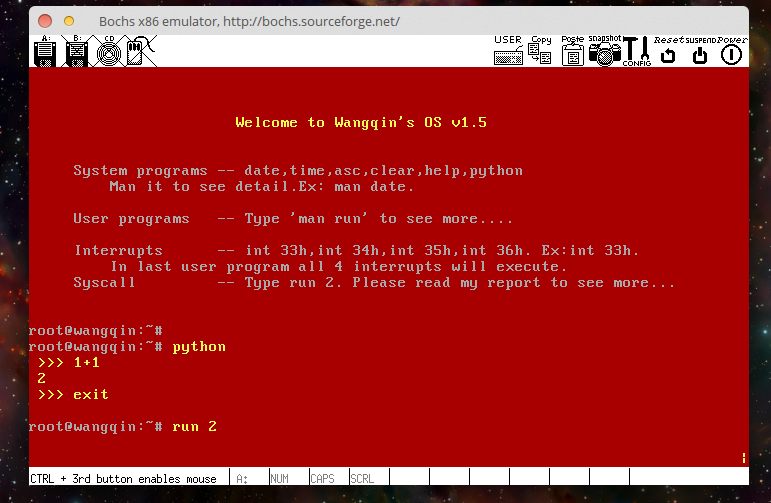
\includegraphics[scale=0.45]{Illustrations/syscall0125.png}}\\\\

下面是第二个用户程序的代码:
{\scriptsize
	\begin{lstlisting}[language={C}]
org 0x1000
;org 0x100

;#0
mov ah,0
int 80h

;LISTEN_EXIT----
listen0:
	mov ah,0
	int 16h


;#2
mov ax,0xb800
mov es,ax
mov dx,1994D
mov ah,2
int 80h

;LISTEN_EXIT----
	mov ah,0
	int 16h

;#1
mov ax,0xb800
mov es,ax
mov dx,1994D
mov ah,1
int 80h

;LISTEN_EXIT----
	mov ah,0
	int 16h



;#5
mov ax,cs
mov ds,ax
mov es,ax

mov cx,0317h  ;position
mov ah,5
mov dx,msg
int 80h


;LISTEN_EXIT----
listen:
	mov ah,0
	int 16h

ret



msg:
	db "hello world!"

times 512-($-$$) db 0	;填充剩余扇区0



	\end{lstlisting}}
下面我们将上面代码分解一下,详细介绍。\\\\
5.1 首先执行执行\verb|ah=0|的系统调用将\verb| OUCH |  打印在屏幕中间
{\scriptsize
\begin{lstlisting}[language={C}]
org 0x1000
;org 0x100

;#0
mov ah,0
int 80h
;LISTEN_EXIT----
listen0:
	mov ah,0
	int 16h

	\end{lstlisting}}
{\center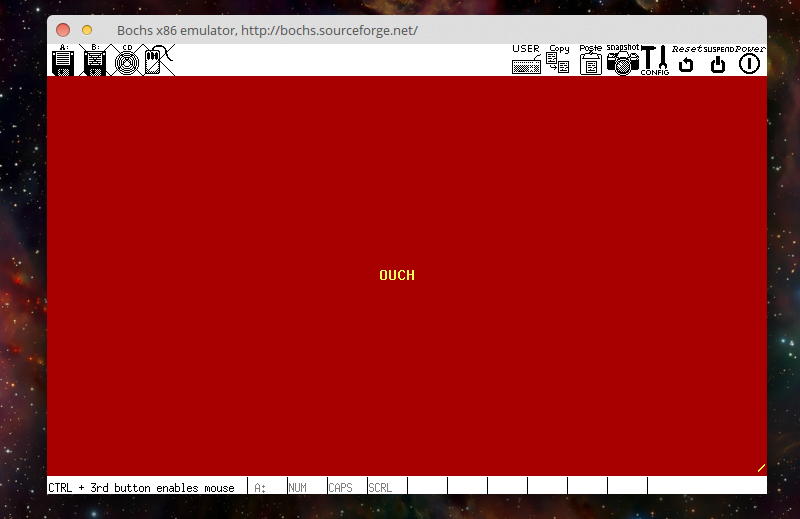
\includegraphics[scale=0.45]{Illustrations/syscall0.png}}\\\\
5.2 现在按下任意键,将执行\verb|ah=2|的系统调用把\verb| OUCH|的第一个字母大写O变成小写o\\\\
{\scriptsize
\begin{lstlisting}[language={C}]
;#2
mov ax,0xb800
mov es,ax
mov dx,1994D
mov ah,2
int 80h

;LISTEN_EXIT----
	mov ah,0
	int 16h

	\end{lstlisting}}
{\center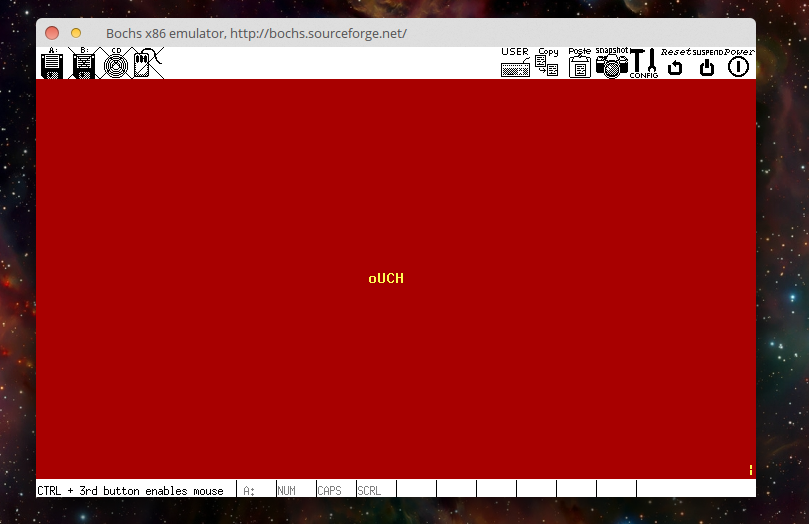
\includegraphics[scale=0.45]{Illustrations/syscall2.png}}\\\\
5.3 按下任意键,执行\verb|ah=1|的系统调用把\verb| oUCH|的第一个字母小写o变回大写O\\\\
{\scriptsize
\begin{lstlisting}[language={C}]
;#1
mov ax,0xb800
mov es,ax
mov dx,1994D
mov ah,1
int 80h

;LISTEN_EXIT----
	mov ah,0
	int 16h


	\end{lstlisting}}
{\center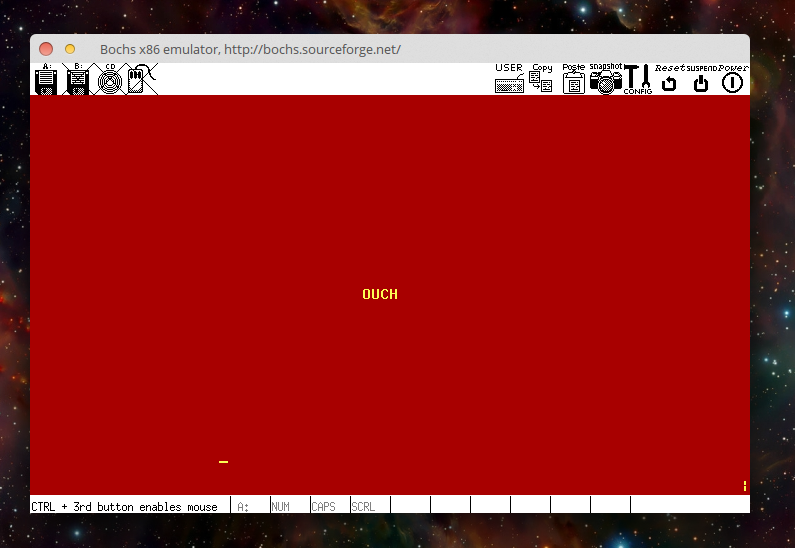
\includegraphics[scale=0.45]{Illustrations/syscall1.png}}\\\\
5.4 按下任意键,执行\verb|ah=5|的系统调用在屏幕3行17列的位置打印一个\verb|helloworld|
{\scriptsize
\begin{lstlisting}[language={C}]
;#5
mov ax,cs
mov ds,ax
mov es,ax

mov cx,0317h  ;position
mov ah,5
mov dx,msg
int 80h


;LISTEN_EXIT----
listen:
	mov ah,0
	int 16h

ret

msg:
	db "hello world!"
	\end{lstlisting}}

{\center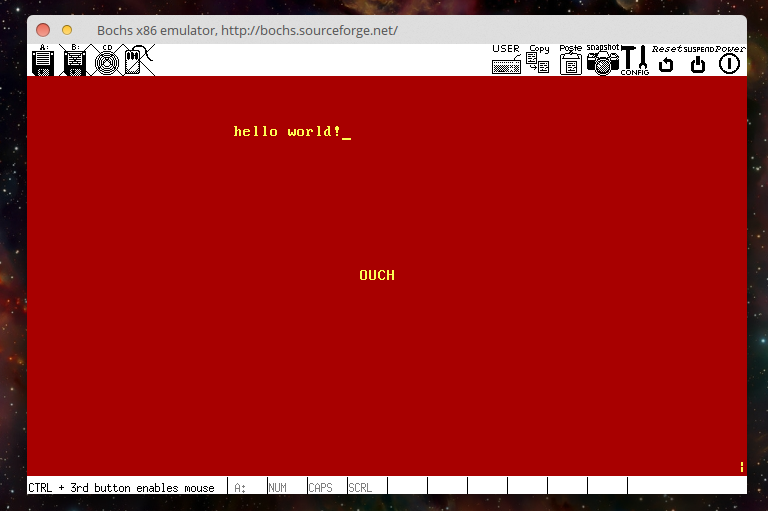
\includegraphics[scale=0.45]{Illustrations/syscall5.png}} \\\\
\indent 5.5 返回操作系统\\\\

6. 内核也有设置自定义中断,在\verb| terminal| 的右下角一直有个横杠在转动,转动频率由\verb| 0x1c|时钟中断触发。在第一个用户程序中\verb| run 1|可以看到自定义的\verb| 33h~36h|中断分别向屏幕1/4位置打印,组合成一个万字旗
{\center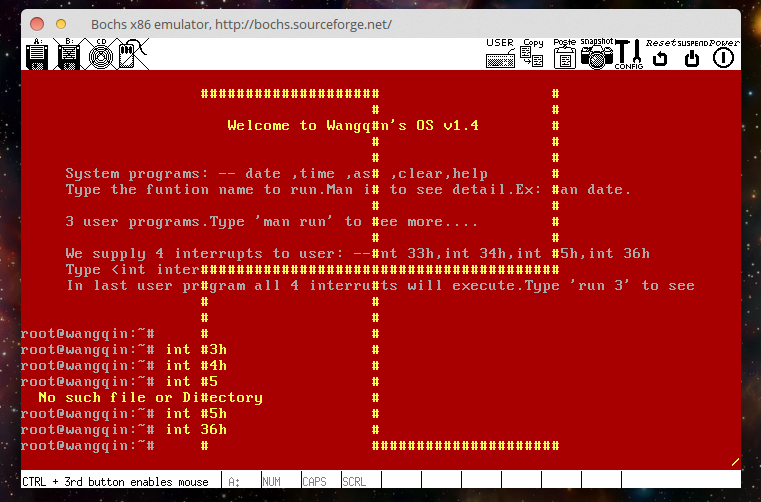
\includegraphics[scale=0.45]{Illustrations/allcustomint.png}}\\\\
{\center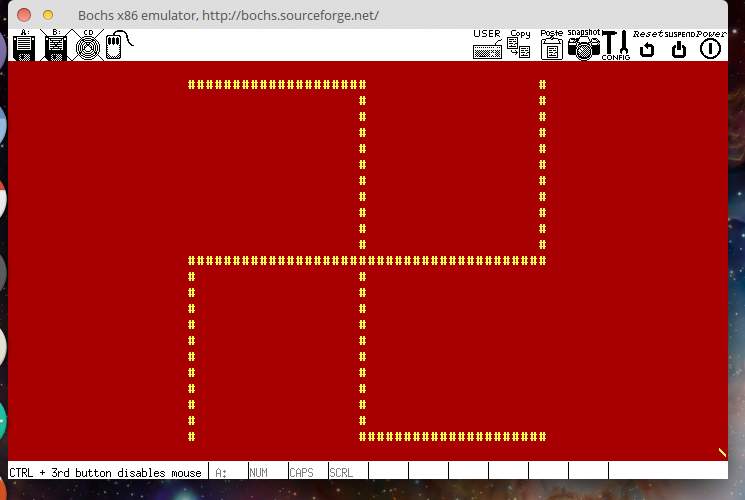
\includegraphics[scale=0.45]{Illustrations/usr2.png}}\\\\

7. 接下来展示这次实验要求实现的多进程调度。\\\\
\indent 7.1 我这里创建并执行进程由命令\verb| start|  触发.
{\center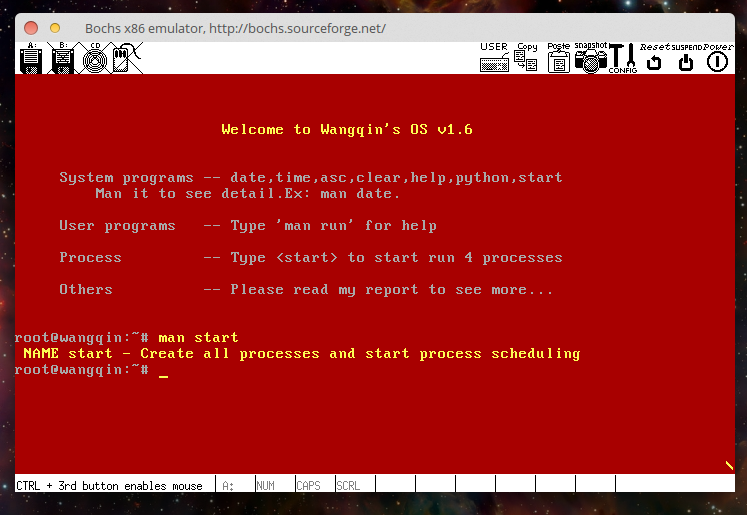
\includegraphics[scale=0.45]{Illustrations/man_start.png}}\\\\
7.2 我们在\verb| terminal|中输入\verb| start|回车。开始创建四个进程并且进行每\verb| 18.2|次的调度,四个进程均分时间片T\\
\[ T = \frac{1 \ S}{18.2} = 0.05494 S = 54.94 ms \]\\\\
{\center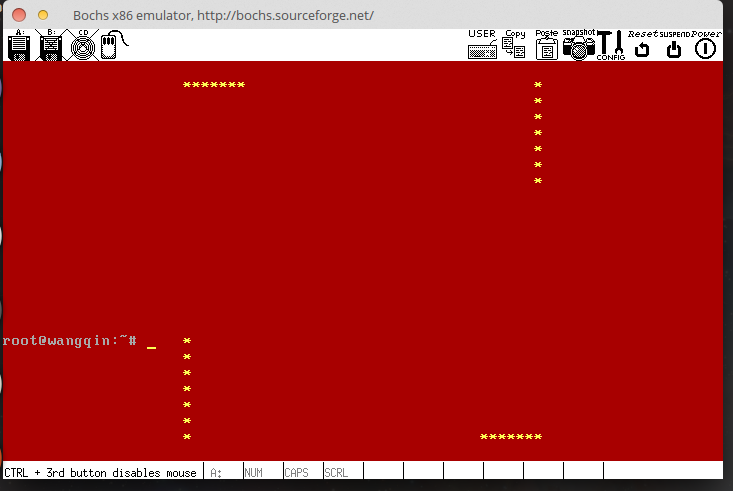
\includegraphics[scale=0.45]{Illustrations/process_start.png}}\\\\
7.3 可以看到每个进程向屏幕四分之一区域打印个性化信息,由于使用的延时函数是用暴力循环的方法,所以存在在不同配置的虚拟机上动画的速度不一样的问题。
{\center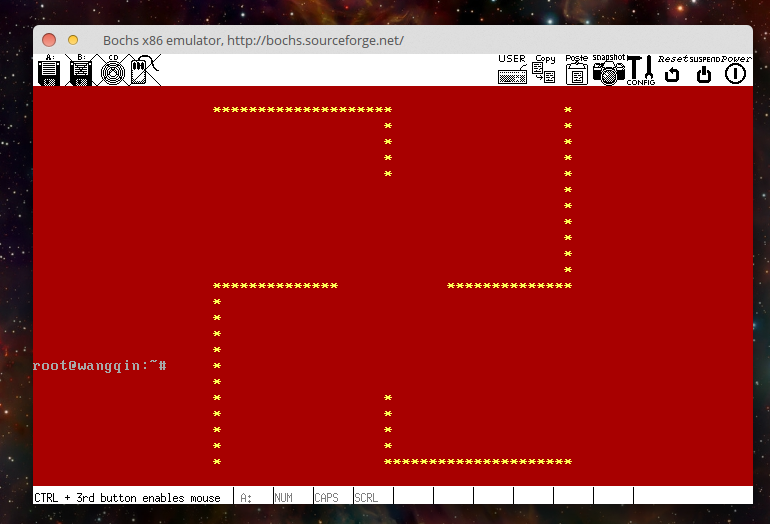
\includegraphics[scale=0.45]{Illustrations/process_start2.png}}\\\\
7.4 在屏幕形成一个万字旗,并且打印出\verb| THE SECOND WORLD WAR| 
{\center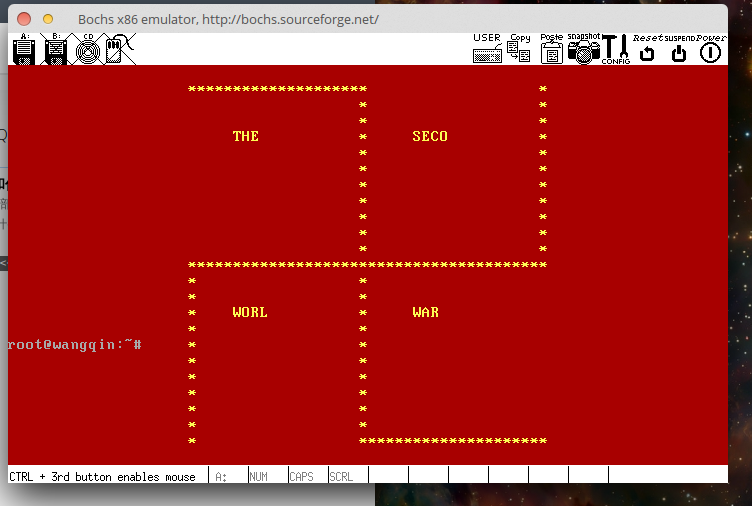
\includegraphics[scale=0.45]{Illustrations/process_start3.png}}\\\\
{\center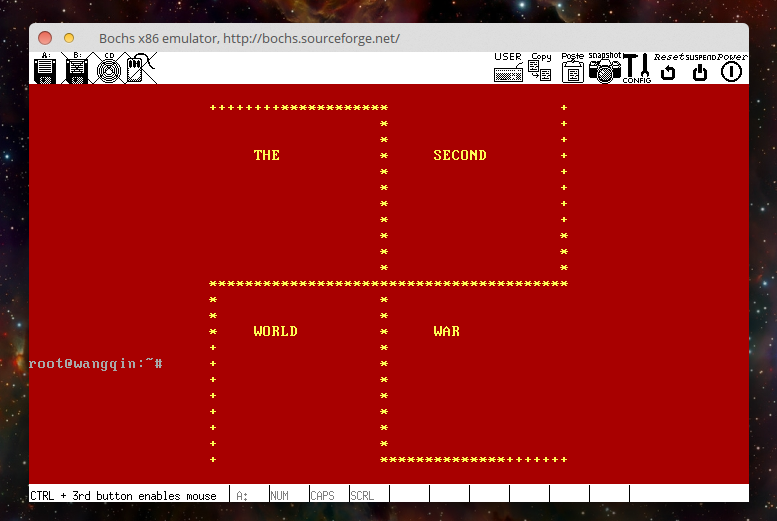
\includegraphics[scale=0.45]{Illustrations/process_start5.png}}\\\\
7.5 进程执行动画描述: 万字旗组成的符号每次循环都被自动加1并显示,直到加到\verb| ascii|码中最后一个字符\verb| ~|,再换回*,如此反复循环\ldots
{\center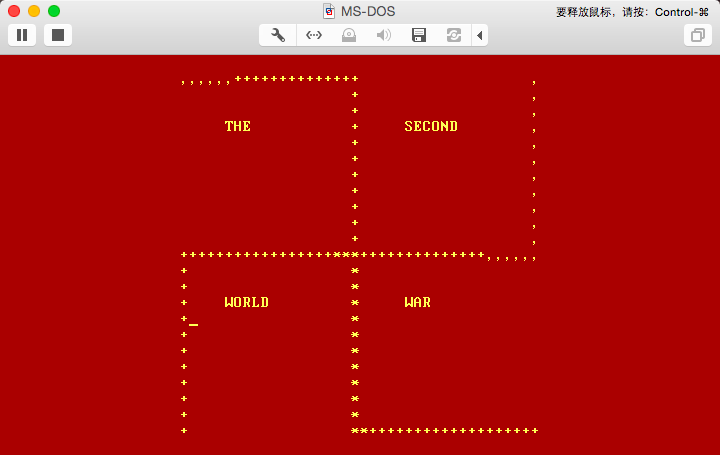
\includegraphics[scale=0.45]{Illustrations/process_1.png}}\\\\
{\center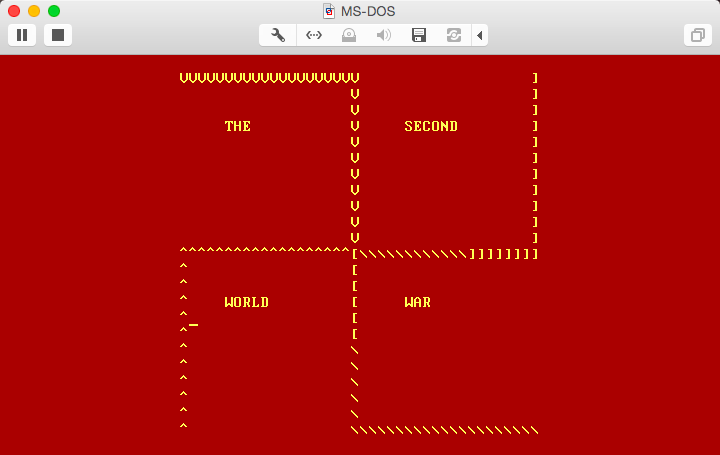
\includegraphics[scale=0.45]{Illustrations/process_2.png}}\\\\
{\center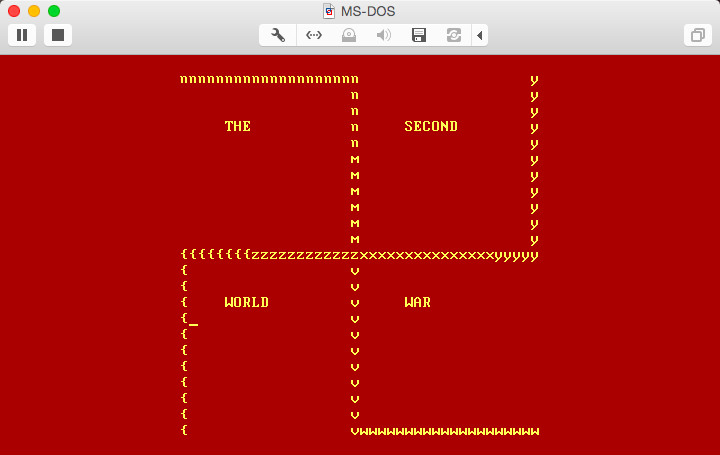
\includegraphics[scale=0.45]{Illustrations/process_3.png}}\\\\
7.6 实际上执行\verb| start| 命令后,总共创建了5个进程,其中四个在上面已经说到,另外一个是为了退出进程调度动画回到\verb| terminal|的监听键盘事件的后台进程。与其他四个进程拥有同样长的时间片,也就是说在进程调度动画执行的任何时候都可以随便按一个键返回\verb| terminal|.
{\center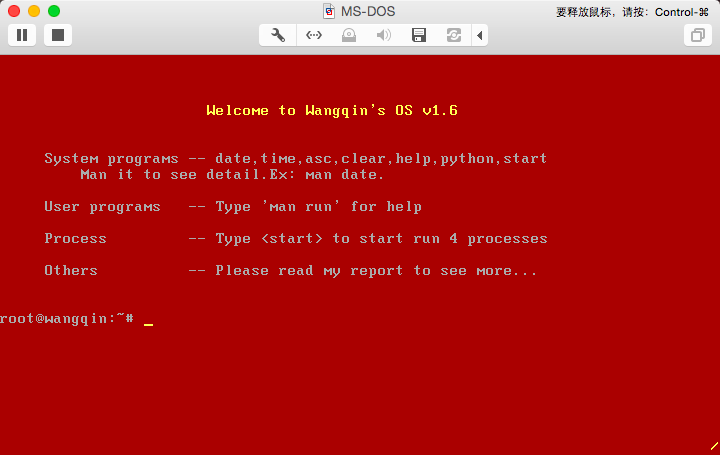
\includegraphics[scale=0.45]{Illustrations/back.png}}\\\\




\section*{ 内存和软盘存储管理}
\hangindent=4em \hangafter=-50{
1. 引导程序加载到内存0x7c00处运行\\
2. 引导程序将操作系统加载到0x7e00处运行\\
3. 操作系统讲用户程序加载到0x1000处运行\\
4. 软盘第1个柱面的第一个扇区存储操作系统引导程序\\
5. 软盘第1个柱面剩下所有扇区2~36扇区存储操作系统内核\\
6. 软盘第\verb|2,3,4,5,6|柱面分别存储五个进程代码\\
7. 软盘第\verb|7,8|柱面分别存储两个用户程序的程序代码\\\\
{\large 栈结构}\\
	\indent 内核栈:从内存的\verb| 0xffff|开始向下扩展\\
	\indent 用户栈:从内存的\verb| 0x1000|开始向下扩展\\
	\indent 进程栈:第i个进程对应的进程栈从内存的\verb| i*0x1000|开始向下扩展\\\\
更多细节信息请阅读我的Makefile文件
}
\section*{ 系统架构}
\hangindent=4em \hangafter=-50{
{\scriptsize 
  \setmonofont{Lantinghei SC Extralight}
\begin{verbatim}
.
├── bochsrc
├── boot.asm				引导程序
├── disk.img
├── kernel                  目录中存放内核相关代码
│   ├── os.asm              主要为os.c提供函数实现.
│   ├── os.c                为内核主要控制模块
│   ├── osclib.c            主要为os.c提供函数实现.
│   ├── os.h
│   ├── oslib.asm           为osclib.c提供更底层的函数封装
│   ├── os_syscall.asm      初始化系统调用和设置系统调用相关模块
│   ├── pcb.h
│   ├── process.c           进程调度创建相关代码
│   ├── terminal.c          装载shell的工具
│   └── terminal.h
├── Makefile                makefile 文件
├── osclib_share.c          内核和用户的共享库(使用户程序体积减少)。
├── oslib_share.asm         内核和用户的共享库(使用户程序体积减少)。
├── process1.asm            第一个进程
├── process2.asm            第二个进程
├── process3.asm
├── process4.asm
├── process_wait_key.asm    监听退出进程
├── python_extension.c      Python扩展
├── README					
├── snapshot.txt
├── stack.png
├── usr1.asm                用户代码
├── usr2.asm

1 directory, 28 files
\end{verbatim}}
}

\setmonofont{Courier New}

\section*{ 主要函数模块}
\hangindent=4em \hangafter=-50{

	1. \verb|os.c: main| 函数模块,由于每次调用汇编函数c都会向栈里面压两个字,但ret返回的时候却只从栈里面弹出一个字,为了保持栈中无冗余数据故每次调用汇编函数都要手动再pop出来一个字。
{\scriptsize\begin{lstlisting}[language={C}]
#include "os.h"			  //include some extern function declare

//============================+MAIN==============
void main(){
	//--------------------init
	screen_init();
	__asm__("pop %si");
	interrupt_init();
	__asm__("pop %si");
	syscall_init();
	__asm__("pop %si");
	print_welcome_msg();
	__asm__("pop %si");
	print_message();
	__asm__("pop %si");
	print_flag(); //root@wangqin4377@:   position
	__asm__("pop %si");
	//--------------------init_end
	while(1){							
		char length = listen_key();// load shell and enter terminal

		if_screen_scroll(); //bottom of screen		
		flag_scroll();//move flag to next line
		__asm__("pop %si");
		if( Print_flag_mark)
			print_flag();
		__asm__("pop %si");
	}
}

//============================MAIN END===============


 \end{lstlisting}}
	2. 为了实现系统调用的工作,故在 os.asm中实现了下列函数供设置系统调用使用,系统调用表在\verb| 0xfe00|的内存位置,\verb| ecx| 为实现系统调用功能的函数内存地址。\verb| ah|为系统调用号码
{\scriptsize
	\begin{lstlisting}[language={C}]
	setting_up_syscall:
	mov bx,0
	mov es,bx
	mov al,ah
	mov ah,0
	shl al,2
	mov bx,0xfe00
	add bx,ax
	mov [es:bx],ecx
	ret
	\end{lstlisting}}
   3. 为了方便自定义中断,在os.asm中实现以下函数。\verb| interrupt_num|是中断号码。eax中存放着中断处理程序
{\scriptsize
	\begin{lstlisting}[language={C}]
insert_interrupt_vector:
	mov ax,0
	mov es,ax
	mov bx,[ interrupt_num]
	shl bx,2 ;interrupt num * 4 = entry
	mov ax,cs
	shl eax,8  ;shl 8 bit   *16
	mov ax,[ interrupt_vector_offset]
	mov [es:bx], eax
ret
\end{lstlisting}}
4. 开机设置系统调用
{\scriptsize
	\begin{lstlisting}[language={C}]
syscall_init:

;----#0 syscall
mov ah,0
mov ecx,0
mov cx,display_center_ouch
call setting_up_syscall

;----#1 syscall
mov ah,1
mov ecx,0
mov cx,letter_upper
call setting_up_syscall

;----#2 syscall
mov ah,2
mov ecx,0
mov cx,letter_lower
call setting_up_syscall

;----#3 syscall
mov ah,3
mov ecx,0
mov cx,atoi_syscall
call setting_up_syscall

;----#4 syscall
mov ah,4
mov ecx,0
mov cx,itoa_syscall
call setting_up_syscall

;----#5 syscall
mov ah,5
mov ecx,0
mov cx,display_str
call setting_up_syscall
ret
	\end{lstlisting}
  }
  5. 设置自定义中断处理程序,第一个设置的就是在terminal右下角不断旋转的小球,原理是使用IRQ0(\verb| 0x08|号中断)
  自动触发的\verb| 0x1C|号中断实现.
  {\scriptsize \begin{lstlisting}[language={C}]

	;#1  setting up time interrupt 
	mov ax,0x1c
	mov [ interrupt_num], ax
	mov ax, timer_interrupt_process
	mov [ interrupt_vector_offset],ax
	call insert_interrupt_vector



	;#2 int 33
	mov ax,0x33
	mov [ interrupt_num], ax
	mov ax, process_int33
	mov [ interrupt_vector_offset],ax
	call insert_interrupt_vector
	
	;#3 int 34
	mov ax,0x34
	mov [ interrupt_num], ax
	mov ax, process_int34
	mov [ interrupt_vector_offset],ax
	call insert_interrupt_vector

	;#4 int 35
	mov ax,0x35
	mov [ interrupt_num], ax
	mov ax, process_int35
	mov [ interrupt_vector_offset],ax
	call insert_interrupt_vector

	;#5 int 36
	mov ax,0x36
	mov [ interrupt_num], ax
	mov ax, process_int36
	mov [ interrupt_vector_offset],ax
	call insert_interrupt_vector

	;#5 int 36
	mov ax,0x80
	mov [ interrupt_num], ax
	mov ax, process_int80
	mov [ interrupt_vector_offset],ax
	call insert_interrupt_vector

	\end{lstlisting}}
  6. 执行用户程序,通过执行run函数自动把terminal中输入指定的用户程序加载到\verb| 0x1000|,并跳转到这里开始执行.
  {\scriptsize \begin{lstlisting}[language={C}]
inline void run( char *str){
	str += 4;
	
	while( *str != '\0'){
	if('0'<*str && *str< Usr_num){
	
			load_user( 5 + *str-'0', 0x1000);	//in oslib.asm	usri in i sector 
			__asm__(" pop %ax");
			run_user();
			__asm__(" pop %ax");
			}else{
				run_error();
				return;
			}
		str++;
	}
	init_flag_position();	
	screen_init();
	print_welcome_msg();
	print_message();
	print_flag(); //root@wangqin4377@:   position
}

	\end{lstlisting}}
 7. 创建进程,首先初始化5个进程(其中有一个是后台监听退出进程),然后分别加载5个进程到相应的内存单元,设置\verb|isProcesRun=1 |用来表示当前正在运行多进程调度,
 让时钟中断的处理程序选择调度的代码执行而不是原来的打印横杠转动的代码。
  {\scriptsize \begin{lstlisting}[language={C}]
void Process(){
	int current_process_SEG = process_SEG;
	int i;
	for( i = 1; i <= process_num_MAX; i++){
		current_process_SEG += 0x1000;
		init_pcb( i, current_process_SEG);	
	}
	load_user(1, 0x1000);
	load_user(2, 0x2000);
	load_user(3, 0x3000);
	load_user(4, 0x4000);
	load_user(5, 0x5000);
	w_is_r=0;
	isProcessRun=1; // enter user process mode
}

	\end{lstlisting}}
 8. 进程调度,这个是本次试验最核心的要求,\verb| w_is_r:which process is running|,\verb| nw_is_r:which next process will run |换老进程下来的时候首先保存的是通用寄存器到这个进程的上下文\verb| TSS|,具体实现就是先把\verb| ax,bx..|等通用寄存器保存到c语言中定义的全局变量中然后再由全局变量保存到进程控制模块队列的pcb结构体中。最后保存的是\verb| IP,CS,Flags,SP|,前三个直接从当前栈中直接pop出来即可,因为cpu在发生中断的时候已经自动把这三个push到栈中了,最后再保存sp,栈指针寄存器。接下来根据\verb| di|寄存器的值来判断是否该结束调度程序回到terminal。如果不是则继续换上新的进程,首先还原的是\verb| sp,ip,cs,flags|,后三个直接push到栈里面就可以了,iret的时候会自动取出来并跳转到\verb| cs:ip|位置执行。最后跳转到\verb| schedule_end|中执行iret结束本次调度。
  {\scriptsize \begin{lstlisting}[language={C}]
void schedule(){
	saveall_reg();			//hurry not inclue sp	
	__asm__("pop %cx");
	__asm__("pop %eax");	//junk

	nw_is_r = w_is_r + 1;
	if( nw_is_r > process_num_MAX){
		nw_is_r = 1;	
	}

	
	saveToqueue();			//code order don't change	


	//----------------set ip cs flag--------
	__asm__("pop %ax");
	__asm__("pop %bx");
	__asm__("pop %cx");

	saveall_reg_seg();		//include sp
	__asm__("pop %cx");

	if( _di == 0x1234){	
		isProcessRun = 0;			//shut down process
		nw_is_r = 0;
		backto_os();
	}else{
		isProcessRun = 1;
	}


	PCB_queue[ w_is_r].tss.SP = _sp;
	PCB_queue[ w_is_r].tss.IP = _ip;
	PCB_queue[ w_is_r].tss.CS = _cs;
	PCB_queue[ w_is_r].tss.Flags = _flags;

		//-----------------end------------------
	_ip = PCB_queue[ nw_is_r].tss.IP;
	_cs = PCB_queue[ nw_is_r].tss.CS;
	_flags = PCB_queue[ nw_is_r].tss.Flags;
	_sp = PCB_queue[ nw_is_r].tss.SP;

	restore_reg_seg();
	__asm__("pop %cx");


	queueTodata();		// ax bx cx...
	
	w_is_r++;
	if( w_is_r > process_num_MAX){
		w_is_r = 1;
	}

	restore_reg();	
	__asm__("pop %di");		//don't use di in any process is dangerous

	__asm__("jmp schedule_end");
	while(1);
}
	\end{lstlisting}}
9. 保存的时候将全局变量的数据保存到pcb中,还原的时候倒过来赋值就可以了。 全局变量实际上就相当于寄存器和pcb之间的一个缓存。
{\scriptsize \begin{lstlisting}[language={C}]
inline void saveToqueue(){
	PCB_queue[ w_is_r].tss.ES = _es;
	PCB_queue[ w_is_r].tss.DS = _ds;
	PCB_queue[ w_is_r].tss.GS = _gs;
	PCB_queue[ w_is_r].tss.FS = _fs;
	PCB_queue[ w_is_r].tss.SS = _ss;
								
	PCB_queue[ w_is_r].tss.AX = _ax;
	PCB_queue[ w_is_r].tss.BX = _bx;
	PCB_queue[ w_is_r].tss.CX = _cx;
	PCB_queue[ w_is_r].tss.DX = _dx;
	PCB_queue[ w_is_r].tss.SI = _si;
	PCB_queue[ w_is_r].tss.DI = _di;
	PCB_queue[ w_is_r].tss.BP = _bp;
}
\end{lstlisting}}
10. 时钟中断处理程序,判断\verb| isProcessRun| 是否为0来决定该执行进程调度程序还是在terminal的右下角显示转动的横杠。

{\scriptsize \begin{lstlisting}[language={C}]
timer_interrupt_process:
	push ax
	mov ax,0
	mov ds,ax
	mov byte al,[ isProcessRun]
	mov ah,0
	cmp al,ah
	je print_corner
	pop ax
	jmp schedule
\end{lstlisting}}
11. 保存寄存器数据到全局变量
{\scriptsize \begin{lstlisting}[language={C}]
extern _ax,_bx,_cx,_dx,_es,_ds,_sp,_bp,_si,_di,_fs,_gs,_ss
saveall_reg:
	mov [_es],es
	mov [_ds],ds
	mov [_gs],gs
	mov [_fs],fs
	mov [_ss],ss

	mov [_ax],ax
	mov [_bx],bx
	mov [_cx],cx
	mov [_dx],dx
	mov [_di],di
	mov [_si],si
	mov [_bp],bp
ret
\end{lstlisting}}
12. 还原\verb| ip,cs,flags| 寄存器数据和切换进程栈。切换进程栈的时候一定要非常小心不要因为函数调用的问题而在切换的时候出现漏洞,否则调度将会失败。
{\scriptsize \begin{lstlisting}[language={C}]
	restore_reg_seg:
	mov ax,[ _ip]
	mov bx,[ _cs]
	mov cx,[ _flags]

	pop si			;ret
	pop di

	mov sp,[ _sp]

	push cx		;flags
	push bx		;cs
	push ax		;ip

	push di
	push si
ret

\end{lstlisting}}


}	
\section*{ 实验心得及仍需改进之处}
\hangindent=4em \hangafter=-50{
	{\large 实验心得:}\\\\
	\indent	本次实验过程中遇到了很多挫折,最大的一个问题就是编写进程调度的算法的时候由于自己疏忽在创建进程启动进程调度的时候没有把时钟中断清零导致,无法发生下一次时钟中断,原本以为 \verb|0x1c|用户时钟中断可以不需要像\verb|0x08|那样每次对\verb|8259|芯片进行重新设置。时钟中断正常工作后又发现调度出现一些问题,比如第一个进程的时间片用完之后不能换到第二个进程执行,当然这个问题还是经过调试很容易解决的。\\
	\indent 后来发现第二个进程执行用完时间片后切换到第一个进程时第一个进程无法按照原来停止执行的\verb|cs:ip|处进行执行,这个问题经过调试也是比较容易解决的。最难调试的问题是栈的切换,我这里为每个进程都设置了一个应用程序栈,进程时间片用完之后切换进程的时候进程的上下文数据\verb|RSS|中
	也会包含这个进程所对应的用户程序栈的栈指针。也就是切换进程的时候也要对应用程序栈\verb| ss:sp|进行切换,但是c语言调用汇编的时候是向栈里压两个字,而汇编返回c调用处的时候是从栈里弹出一个字到\verb| IP|指令指针寄存器。\\
	\indent 这种不对称的出栈入栈很容易造成使用栈的过程中导致栈数据混乱。而且当时钟中断的处理程序即进程调度程序执行完毕后要从栈里弹出三个字的数据到\verb| IP,CS,Flags|这些寄存器,调度的时候就要手动的先把原来的\verb| IP,cs,flags|弹出来保存然后压入新进程的\verb| ip,cs,flags|,所以保持栈清晰,有规律是非常重要的,否则进程调度将会失败。
	\\
	\indent 栈切换这里这里调了很长时间,得到的教训就是一定要注意细节,c调用汇编或汇编调用c都要特别注意有没有冗余的数据被压栈,注意一定要先保存\verb| ip,cs,flags,sp|和一些段寄存器的数据,合适的时机再切换栈指针寄存器。当换一个新进程开始执行的时候一定要保证这个进程上次被换下来的时候,栈指针寄存器\verb| sp|一定是上次的位置减去三个字,因为要压入\verb| ip,cs,flags|。总之注意写代码的时候注意细节总会可以大大降低\verb|debug|的时间从而减少写代码的总时间,提高编程效率。同时也是
	作为一个专业学生好的习惯。这次实验中我优化了操作系统和内核的结构,将\verb| shell|和内核分开,使主内核文件\verb| os.c|代码量大大减少,向\verb|Linux|提倡的微内核走进了一步。\\\\
	{\large 实验仍需改进之处:}\\\\
	\indent 仍需完善细节,比如说\verb|python|的命令行工具加入乘法,除法完全是几行代码的问题\\
	\indent 可以考虑将用户程序做成\verb|elf|格式,动态链接系统的代码库。目前的情况是用户程序自己带着一份和操作系统一样的代码库,分别联合编译\\
	\indent 考虑精简操作系统代码,减少冗余代码\\
	\indent 增加文件系统功能\\
	\indent 调度算法和进程控制模块的存储有待优化\\
	\indent 继续优化调整操作系统内核架构和内存磁盘管理\\
}
\fancyfoot[OC]{ \footnotesize{https://github.com/wangqin4377/Homework\_Wangqin/tree/master/OS\_homework/}}
\end{document}

